\chapter{Dữ liệu chính phủ}
\label{ch:M1L2}

\section*{Lesson Notes}
\section[Dữ liệu Kinh tế và Tài chính]{Dữ liệu Kinh tế và Tài chính (Economics and Financial Data)}

Giá cả tài sản bị ảnh hưởng rất lớn bởi những gì diễn ra trong nền kinh tế vĩ mô. Một chu kỳ kinh doanh bùng nổ sẽ thu hút đầu tư vốn cổ phần, làm tăng chi tiêu cá nhân, và có thể dẫn đến các hành động từ ngân hàng trung ương. Trong module đầu tiên về Thị trường Tài chính, bạn đã thấy các ví dụ trong đó người gửi tiền hưởng một mức lãi suất cụ thể. Cùng lúc đó, người cho vay (hoặc người đi vay) lại chịu một mức lãi suất khác. Gửi tiền vào ngân hàng chắc chắn sẽ mang lại mức tiền lãi thấp hơn so với tiền lãi bạn phải trả cho một khoản vay từ chính ngân hàng đó!

Một trong những yếu tố ảnh hưởng lớn nhất đến thị trường nói chung, và lãi suất nói riêng, là tin tức. Tin tức có thể được coi là nằm trong dự kiến (expected) hoặc ngoài dự kiến (unexpected). Hãy nhớ lại rằng các thị trường hiệu quả có thể đã phản ánh phần lớn các tin tức dự kiến vào giá. Ví dụ, giả sử Netflix tuyên bố trả cổ tức \$2.00. Nếu đây thực sự là con số được công bố, thì nó không gây ngạc nhiên và sẽ không ảnh hưởng đến giá cổ phiếu của Netflix. Tuy nhiên, giả sử có tin tức ngoài dự kiến.

\begin{itemize}
    \item Netflix có sự tăng trưởng mạnh hơn dự đoán do đánh giá thấp mức độ phổ biến của một số chương trình, dẫn đến số lượng người đăng ký tại Hàn Quốc lớn hơn dự kiến. Mức cổ tức là \$2.40. Giá cổ phiếu có khả năng sẽ tăng vọt.
    \item Mặt khác, giả sử Netflix có chi phí sản xuất nội dung gốc cao hơn dự kiến, khiến lợi nhuận ròng sụt giảm. Cổ tức chỉ còn \$1.80. Giá cổ phiếu có khả năng sẽ lao dốc.
\end{itemize}

Tin tức ngoài dự kiến có thể là tin tốt hoặc tin xấu; tức là, nó có thể dẫn đến giá cao hơn hoặc giá thấp hơn, tùy thuộc vào tình hình. Ví dụ, hãy xem xét tin xấu. Nó có thể làm tăng rủi ro tín dụng, đe dọa dòng tiền tài trợ, tạo ra sự biến động, phá vỡ mối tương quan, làm trầm trọng thêm đòn bẩy, gây ra tính phi tuyến, thách thức các giả định của mô hình, gây áp lực lên các mô hình bằng cách phát sinh thêm chi phí cho thanh khoản, thúc đẩy sự thất bại của mô hình, và thậm chí mang lại các cuộc khủng hoảng tài chính. Tất nhiên, một mẩu tin xấu có thể không gây ra tất cả những điều đó, nhưng sẽ ra sao nếu tin xấu ảnh hưởng đến nhiều doanh nghiệp, chẳng hạn như lãi suất cao hơn dự kiến?

Hãy xem xét cách thức hoạt động của lãi suất. Đầu tư vào kinh doanh ảnh hưởng đến lãi suất, nhưng đồng thời, lãi suất cũng ảnh hưởng đến các khoản đầu tư kinh doanh. Hầu hết các mối quan hệ trong tài chính đều phức tạp vì chúng có thể mang tính đa chiều. Không chỉ là A ảnh hưởng đến B và B ảnh hưởng đến A. Mà là A ảnh hưởng đến B và C; B ảnh hưởng đến A và C; C ảnh hưởng đến A và B; và cứ tiếp tục như vậy. Ví dụ, nếu chúng ta chỉ thu thập lãi suất mà không có ý niệm gì về chính sách tiền tệ, cung tiền hay các quyết định kinh tế, chúng ta sẽ đánh mất đi dữ liệu mà vừa ảnh hưởng đến lãi suất lại vừa bị ảnh hưởng bởi chính các mức lãi suất đó. Thực tế, chúng ta có thể muốn thu thập các dữ liệu liên quan để có thể kiểm tra xem các biến số khác (ví dụ: các quyết định của Fed) có ảnh hưởng đến biến số mà chúng ta đang quan tâm hay không.

\section[Cục Dự trữ Liên bang và Tác động của nó]{Cục Dự trữ Liên bang và Tác động của nó (The Federal Reserve and Its Impact)}

Nhớ lại từ môn Thị trường Tài chính rằng chúng ta đã đọc về các ngân hàng trung ương. Cục Dự trữ Liên bang (Federal Reserve - Fed) là ngân hàng trung ương của Hoa Kỳ. Đầu ra của Fed rất rộng lớn: nó bao gồm các quyết định, nghiên cứu, và các bài bình luận thị trường được xuất bản và phát biểu. Những kết quả này được theo dõi và phân tích rất kỹ lưỡng, vì chúng ảnh hưởng đáng kể đến thị trường. Ví dụ, tám lần một năm, Cục Dự trữ Liên bang có lịch trình phát hành thường xuyên các quyết định về lãi suất. Những cuộc họp này dẫn đến các quyết định về lãi suất được công bố ra thị trường. Giống như bất kỳ thông tin nào khác, đây là tin tức có thể nằm trong dự kiến hoặc ngoài dự kiến. Nếu tin tức là trong dự kiến, thì thông tin đó đã được phản ánh vào giá trên thị trường. Nếu tin tức là ngoài dự kiến, thì rất có khả năng sẽ có những cú sốc thông tin gây ra sự biến động trên thị trường. Ngoài ra, Fed còn chọn 8 ngày khác để công bố biên bản các cuộc họp. Những bản phát hành này chứa dữ liệu định tính thay vì định lượng. Các bản công bố này cũng có thể ảnh hưởng không chỉ đến lãi suất mà còn đến giao dịch chứng khoán, vì chúng chỉ ra ý kiến và hành động dự kiến của Fed. Ví dụ, vào năm 2019, Fed đã quyết định cắt giảm lãi suất ba lần. Điều này đã dẫn đến mức tăng 29\% của chỉ số S\&P 500 trong quý 4 năm 2019.

Nếu chúng ta thu thập dữ liệu trong năm 2018 và sau đó cố gắng ngoại suy, chúng ta sẽ bỏ lỡ các sự kiện chính ảnh hưởng đến dữ liệu. Thường thì, chúng ta cần phải hiểu các sự kiện chính tác động đến dữ liệu của mình, vì chúng ta có thể coi một mẫu dữ liệu là thông tin giữa các sự kiện đó. Ví dụ, nếu bạn xây dựng một mẫu dữ liệu vốn cổ phần, bạn có thể thu thập giá đóng cửa của cổ phiếu hàng ngày, nhưng khi tiến hành phân tích chúng, bạn có thể xem xét:
\begin{enumerate}
    \item không phân nhóm
    \item 1 nhóm cho mỗi lần thông báo cổ tức của cổ phiếu
    \item phân nhóm dựa trên mức lãi suất của Cục Dự trữ Liên bang
    \item 1 nhóm cho mỗi cuộc họp quỹ Fed
\end{enumerate}

Mặc dù dữ liệu thu thập được có thể giống nhau, nhưng có một sự thừa nhận rằng toàn bộ dữ liệu (ví dụ 1) có thể có các đặc tính khác nhau và có thể được phân tích tốt hơn dựa trên thuộc tính nội tại của công ty (ví dụ 2, thu nhập) hoặc dựa trên thuộc tính bên ngoài, như chính sách tiền tệ (ví dụ 3 và 4). Hiểu được rằng dữ liệu của chúng ta trải qua sự thay đổi đồng nghĩa với việc chúng ta sẽ muốn hiểu các thị trường như những hệ thống. Điều đó cũng có nghĩa là chúng ta có thể muốn thu thập và phân tích các dữ liệu mang tính định tính (ví dụ: các tuyên bố của Fed).

\section[Dữ liệu Chính phủ là gì?]{Dữ liệu Chính phủ là gì? (What is Government Data?)}

Dữ liệu chính phủ là tất cả những thông tin được thu thập bởi các thực thể chính phủ. Dữ liệu này bao gồm:
\begin{itemize}
    \item Dữ liệu Kinh tế (GDP, lạm phát, tỷ lệ việc làm, v.v.)
    \item Dữ liệu Nhân khẩu học
    \item Dữ liệu Môi trường
    \item Dữ liệu Y tế
    \item Dữ liệu Pháp lý
    \item Dữ liệu Nông nghiệp
    \item Dữ liệu Năng lượng
    \item Dữ liệu Giáo dục
    \item Dữ liệu Bất động sản
\end{itemize}

và nhiều danh mục dữ liệu khác mà một chính phủ cụ thể có thể chọn hoặc không chọn để theo dõi. Dữ liệu trên là rất cần thiết cho mọi cơ chế ra quyết định được chính phủ kết hợp. Ví dụ, đã được xác định rõ dữ liệu kinh tế quan trọng như thế nào đối với chính sách tiền tệ và tài khóa hay dữ liệu y tế đã giúp các cơ quan tương ứng điều phối phản ứng của hệ thống chăm sóc sức khỏe trong đại dịch COVID-19 ra sao.

Về bản chất, dữ liệu này đóng vai trò như sự quản trị dựa trên bằng chứng và cái nhìn toàn diện của chúng cho phép các chính phủ đưa ra các quyết định cho tương lai của một quốc gia trong bối cảnh thực tế phức tạp.

\subsection[Các khía cạnh của Dữ liệu Chính phủ]{Các khía cạnh của Dữ liệu Chính phủ (Aspects of Government Data)}

Tính đến lúc này, chúng ta đã thấy phạm vi của dữ liệu chính phủ, nhưng cũng có những đặc điểm khác:
\begin{itemize}
    \item Khối lượng (Volume): khối lượng dữ liệu chính phủ có xu hướng rất lớn
    \item Đa dạng (Variety): nhiều danh mục dữ liệu có cấu trúc và phi cấu trúc
    \item Thẩm quyền (Authoritative): nó mang tính chính thức (cùng một dữ liệu được sử dụng để hoạch định chính sách)
    \item Tính kịp thời (Timeliness): người ta có thể tìm thấy dữ liệu thời gian thực và dữ liệu lịch sử
    \item Chất lượng (Quality): có thể có những tập dữ liệu không đầy đủ hoặc không chính xác
    \item Định dạng (Format): dữ liệu được lưu trong cơ sở dữ liệu, các tệp (CSV, JSON, v.v.), báo cáo, và các định dạng khác
    \item Độ nhạy cảm/Khả năng tiếp cận (Sensitivity/Accessibility): nó có thể bao gồm thông tin cá nhân, trong trường hợp đó nó sẽ bị hạn chế
    \item Siêu dữ liệu (Metadata): các mô tả của tập dữ liệu đóng vai trò như một bản kiểm kê để điều hướng khối lượng dữ liệu lớn
\end{itemize}

Bổ sung thêm, liên quan đến các đặc điểm trên, đã có một nỗ lực đáng kể từ phía một số chính phủ nhằm thực hiện tính minh bạch và tính mở trong dữ liệu của họ. Những nỗ lực này đã làm nảy sinh Dữ liệu Chính phủ Mở (Open Government Data), mang hình thức của một phong trào thúc đẩy nhiều quốc gia cung cấp quyền truy cập công khai vào dữ liệu của họ.

\subsection[Dữ liệu Chính phủ Mở]{Dữ liệu Chính phủ Mở (Open Government Data)}

Năm 1966, Hoa Kỳ là nước đầu tiên thực hiện chính sách về dữ liệu mở bằng cách thiết lập một khuôn khổ pháp lý mang tên "Đạo luật Tự do Thông tin" (Freedom of Information Act - FOIA). Theo FOIA, bất kỳ công dân nào cũng có thể yêu cầu quyền truy cập công khai vào các hồ sơ từ bất kỳ cơ quan liên bang nào. Nhưng đây là tính minh bạch mang tính "phản ứng" (reactive) vì dữ liệu không được mở theo mặc định. Điều này chỉ được sửa đổi vào năm 2009 bởi Chỉ thị Chính phủ Mở (Open Government Directive), bắt buộc các cơ quan liên bang phải xuất bản thông tin chính phủ trực tuyến và đi theo chính sách chính phủ mở. Đây là bước đi quyết định từ tính minh bạch "phản ứng" sang tính minh bạch "chủ động" (proactive), nơi bất kỳ ai cũng có thể truy cập dữ liệu công cộng mà không cần phải có yêu cầu rõ ràng. Vương quốc Anh cũng ra mắt Sáng kiến Dữ liệu Mở vào năm 2010, tiếp theo là Chỉ thị Dữ liệu Mở của EU vào năm 2019. Các quốc gia khác như Canada, Úc, Ấn Độ và Nhật Bản cũng đã thực hiện các chính sách dữ liệu mở của riêng họ.

Dưới đây là định nghĩa về Dữ liệu Chính phủ Mở như được tìm thấy trong Cổng Dữ liệu Châu Âu (European Data Portal):

Dữ liệu (Chính phủ) Mở đề cập đến thông tin được thu thập, sản xuất hoặc được chi trả bởi các cơ quan công quyền (còn được gọi là Thông tin Khu vực Công) và được cung cấp miễn phí để tái sử dụng cho bất kỳ mục đích nào. Giấy phép sẽ chỉ định rõ các điều khoản sử dụng. Những nguyên tắc đối với Dữ liệu Mở này được mô tả chi tiết trong Định nghĩa Mở (Open Definition).

Tập con này của dữ liệu chính phủ sẽ (một phần) định hướng các tập dữ liệu mà bạn sẽ sử dụng tại WQU. Những tập dữ liệu trong thế giới thực này sẽ giúp bạn phát triển các kỹ năng thực tế trong việc phân tích và lập mô hình dữ liệu, đồng thời mang lại cái nhìn sâu sắc về các chỉ số kinh tế và các yếu tố khác ảnh hưởng đến nền kinh tế. Tóm lại, tính minh bạch trong dữ liệu chính phủ đã làm phong phú thêm nội dung của WQU cũng như toàn bộ quá trình học tập.

\subsection[Dữ liệu Kinh tế của Cục Dự trữ Liên bang]{Dữ liệu Kinh tế của Cục Dự trữ Liên bang (Federal Reserve Economic Data - FRED)}

Một ví dụ điển hình về dữ liệu chính phủ mở đang hoạt động là Dữ liệu Kinh tế của Cục Dự trữ Liên bang (FRED). Hiện tại, FRED nổi bật với tư cách là một trong những cơ sở dữ liệu kinh tế toàn diện và dễ tiếp cận nhất dành cho công chúng. Dữ liệu này được duy trì bởi Ngân hàng Dự trữ Liên bang St. Louis và được đặc biệt quan tâm, phù hợp với các nguyên tắc về tính mở, như một nguồn tài nguyên quan trọng cho các nhà nghiên cứu, các nhà hoạch định chính sách, sinh viên và công chúng.

\subsubsection[Tổng quan về FRED]{Tổng quan về FRED (Overview of FRED)}

FRED là một kho lưu trữ khổng lồ về dữ liệu chuỗi thời gian kinh tế từ nhiều nguồn khác nhau, không chỉ giới hạn trong Hệ thống Dự trữ Liên bang. Nó bao gồm dữ liệu từ:
\begin{itemize}
    \item Các cơ quan chính phủ Hoa Kỳ (ví dụ: Cục Thống kê Lao động, Cục Phân tích Kinh tế)
    \item Các tổ chức quốc tế (ví dụ: Ngân hàng Thế giới, OECD)
    \item Các nguồn tư nhân (ví dụ: các trung tâm nghiên cứu của trường đại học)
\end{itemize}

Cơ sở dữ liệu bao gồm một loạt các chỉ số kinh tế, bao gồm:
\begin{itemize}
    \item Tổng sản phẩm quốc nội (GDP)
    \item Tỷ lệ lạm phát
    \item Thống kê việc làm
    \item Lãi suất
    \item Tỷ giá hối đoái
    \item Chỉ số giá tiêu dùng và nhà sản xuất
    \item Các khối tiền tệ (Monetary aggregates)
\end{itemize}

\subsubsection[Các tính năng chính của FRED]{Các tính năng chính của FRED (Key Features of FRED)}

1. Khả năng tiếp cận: Dữ liệu FRED được cung cấp miễn phí thông qua giao diện web thân thiện với người dùng, các ứng dụng di động và truy cập API.
2. Trực quan hóa Dữ liệu: Người dùng có thể tạo biểu đồ và đồ thị tùy chỉnh trực tiếp trên trang web FRED.
3. Tải xuống Dữ liệu: Dữ liệu có thể dễ dàng được tải xuống dưới nhiều định dạng (ví dụ: Excel, CSV) để phân tích thêm.
4. Cập nhật Thường xuyên: FRED được cập nhật theo thời gian thực khi có dữ liệu mới từ các nguồn của nó.
5. Dữ liệu Lịch sử: Nhiều chuỗi trong FRED có dữ liệu lùi lại vài thập kỷ, cung cấp bối cảnh lịch sử có giá trị.
6. Chuyển đổi Dữ liệu: FRED cho phép người dùng thực hiện các chuyển đổi cơ bản trên các chuỗi dữ liệu, chẳng hạn như thay đổi đơn vị hoặc tính toán phần trăm thay đổi.

Cho mục đích của bài học này, chúng ta sử dụng cổng API để có thể sử dụng các thư viện thống kê và trực quan hóa của Python.

\section[Đường cong Lợi suất]{Đường cong Lợi suất (Yield Curve)}

Trong phần này, chúng ta sẽ làm việc với một loại đường cong lợi suất cụ thể gọi là đường cong lợi suất Trái phiếu Kho bạc Kỳ hạn Không đổi (Constant Maturity Treasury - CMT). Trong môn Thị trường Tài chính, sinh viên đã được giới thiệu về chủ đề này, và chúng ta sẽ bổ sung cho tài liệu đó bằng một quy trình làm việc với dữ liệu thực hành.

Đường cong lợi suất CMT là một bức ảnh chụp nhanh về tất cả lợi suất Trái phiếu Kho bạc Hoa Kỳ tại một ngày nhất định. Về cơ bản, Bộ Tài chính Hoa Kỳ sử dụng lợi suất chào mua trên thị trường lúc đóng cửa (dựa trên mức giá mà người mua sẵn sàng trả (bid) thay vì giá giao dịch thực tế) để tính toán các mức lãi suất CMT hàng ngày. Bạn có thể tìm thấy tổng quan về phương pháp luận mà Bộ Tài chính sử dụng tại đây.

Một cách thuận tiện, FRED đã thực hiện các tính toán này và lãi suất CMT được cung cấp miễn phí từ trang web của họ hoặc thông qua FRED API, mà chúng ta có thể tận dụng thông qua thư viện Python \texttt{fredapi}. Để truy cập dữ liệu FRED, mỗi sinh viên phải lấy một khóa API (API key) bằng cách làm theo các bước sau:
1. Truy cập trang web FRED: https://fred.stlouisfed.org/docs/api/api\_key.html. Nhấp vào "Create an Account" (Tạo tài khoản) ở góc trên cùng bên phải (nếu bạn chưa có tài khoản với FRED).
2. Đăng nhập vào tài khoản FRED của bạn và yêu cầu khóa API. Điều hướng đến mục "API Keys" của menu thả xuống "My Account" ở góc trên cùng bên phải. Sau đó, nhấp vào "Request API Key."

\begin{lstlisting}[language=Python]
In [1]: import pandas as pd
        from fredapi import Fred
        import matplotlib.pyplot as plt
        import seaborn as sns
        sns.set()
\end{lstlisting}

\begin{lstlisting}[language=Python]
In [2]: # Initialize the FRED API with your key
        fred = Fred(api_key='99b15e0a2f3b3f4571893e831fd555d0') # Replace my APIKEY
        
        # List of Treasury yield series IDs
        series_ids = ['DGS1MO', 'DGS3MO', 'DGS6MO', 'DGS1', 'DGS2', 'DGS3', 'DGS5', 
                      'DGS7', 'DGS10', 'DGS20', 'DGS30']
        
        # Function to get data for a single series
        def get_yield_data(series_id):
            data = fred.get_series(series_id, observation_start="1975-01-01", observ
            return data
            
        #Get data for all series
        yields_dict = {series_id: get_yield_data(series_id) for series_id in series_
        
        # Combine into a single DataFrame
        yields = pd.DataFrame(yields_dict)
        
        # Rename columns for clarity
        yields.columns = ['1 Month', '3 Month', '6 Month', '1 Year', '2 Year', '3 Ye
                          '7 Year', '10 Year', '20 Year', '30 Year']
\end{lstlisting}

\begin{lstlisting}[language=Python]
In [3]: yields.index = pd.to_datetime(yields.index)
        yields.loc['2020-01-03']
\end{lstlisting}

\begin{lstlisting}[language=Python]
Out [3]: 1 Month    1.52
         3 Month    1.52
         6 Month    1.55
         1 Year     1.55
         2 Year     1.53
         3 Year     1.54
         5 Year     1.59
         7 Year     1.71
         10 Year    1.80
         20 Year    2.11
         30 Year    2.26
         Name: 2020-01-03 00:00:00, dtype: float64
\end{lstlisting}

Dataframe trên chứa một hàng từ bộ dữ liệu của chúng ta: tất cả các lợi suất CMT tại một ngày cụ thể.
Các mức lợi suất được biểu thị dưới dạng phần trăm. Ví dụ, lợi suất "1 Month" là 1.52, có nghĩa là 1.52\% hoặc 0.0152, và độ chính xác của các mức lợi suất được trình bày là một điểm cơ bản (0.01\%).

\begin{lstlisting}[language=Python]
In [4]: yields.isna().sum(axis = 0)
\end{lstlisting}

\begin{lstlisting}[language=Python]
Out [4]: 1 Month    7180
         3 Month    2204
         6 Month    2204
         1 Year      542
         2 Year      894
         3 Year      542
         5 Year      542
         7 Year      542
         10 Year     542
         20 Year    2231
         30 Year    1072
         dtype: int64
\end{lstlisting}

Điều đầu tiên chúng ta nhận thấy là phần dữ liệu bị thiếu. Một số kỳ hạn như 1 tháng, 3 tháng và 6 tháng không được theo dõi qua thời gian vì trước những năm 2000, trọng tâm chủ yếu nằm ở các kỳ hạn dài hơn. Trái phiếu 20 năm có lịch sử phát hành không đều đặn vì từ năm 1986 đến 1993, T-bonds 20 năm không được phát hành. Điều tương tự cũng áp dụng cho kỳ hạn 30 năm, vốn đã bị ngừng từ tháng 2 năm 2002 đến tháng 2 năm 2006. Hơn nữa, một lượng lớn các giá trị bị thiếu, như ta có thể thấy ở các trái phiếu có tính thanh khoản cao hơn như kỳ hạn 3, 5, 7 và 10 năm, có thể là do các ngày nghỉ lễ và sự gián đoạn của thị trường.

\begin{lstlisting}[language=Python]
In [5]: # We can see that during the days that the 10-year is not reported,
        # none maturity is reported as well.
        yields[yields['10 Year'].isna() == True].sum(axis = 0)
\end{lstlisting}

\begin{lstlisting}[language=Python]
Out [5]: 1 Month    0.0
         3 Month    0.0
         6 Month    0.0
         1 Year     0.0
         2 Year     0.0
         3 Year     0.0
         5 Year     0.0
         7 Year     0.0
         10 Year    0.0
         20 Year    0.0
         30 Year    0.0
         dtype: float64
\end{lstlisting}

Hãy vẽ biểu đồ lợi suất cho tất cả các ngày khả dụng. Mặc dù bộ dữ liệu của chúng ta chỉ trở nên "hoàn chỉnh" sau những năm 2000, việc quan sát cách lãi suất tiến triển qua thời gian vẫn rất quan trọng.

\begin{lstlisting}[language=Python]
In [6]: # Figure 1
        yields.plot(figsize=(12,8), title='Treasury Yields', alpha=0.7) # Plot the 
        plt.show()
\end{lstlisting}

\begin{figure}[htbp]
    \centering
    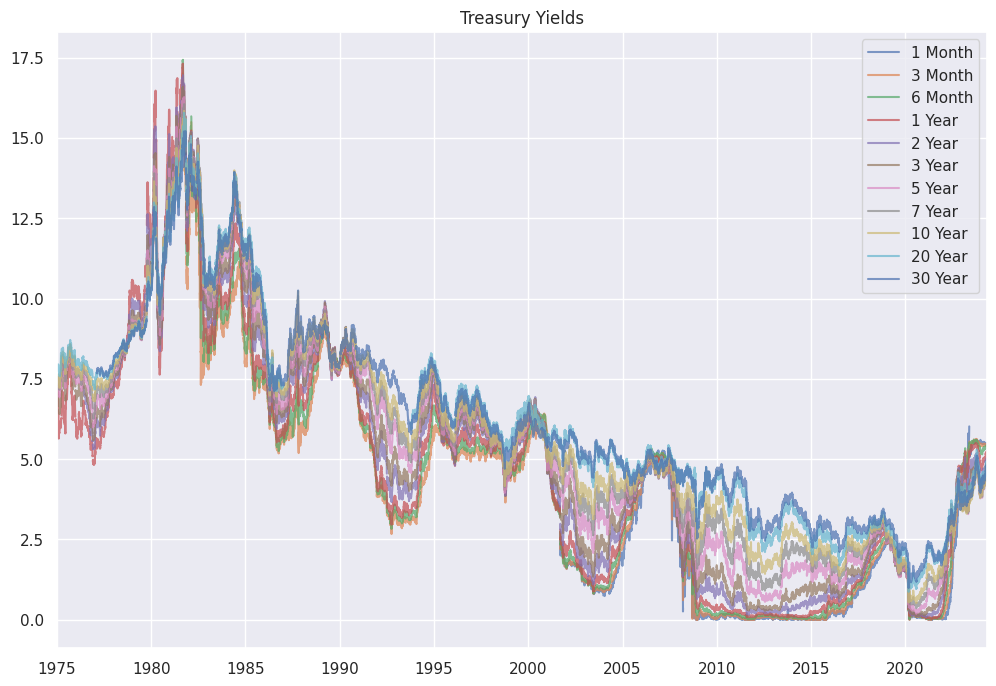
\includegraphics[width=1\textwidth]{gfx/m1l2_notes_fig1_treasury_yields.png}
    \caption{Lợi suất Trái phiếu Kho bạc qua các năm (1975 - nay)}
    \label{fig:m1l2_notes_fig1_treasury_yields}
\end{figure}

Bài tập 1
Liệt kê tất cả các cuộc suy thoái kinh tế của Hoa Kỳ sau năm 1975. Bạn quan sát thấy điều gì về các mức lãi suất trong các cuộc suy thoái này? Sử dụng đồ thị ở trên để lập luận về cách lãi suất biến động trong thời kỳ suy thoái kinh tế. Để làm cho mọi thứ rõ ràng hơn, bạn có thể chọn một hoặc hai cuộc suy thoái của Hoa Kỳ và vẽ lại biểu đồ trên chỉ trong thời gian xảy ra khủng hoảng (và một vài năm trước và sau năm khủng hoảng).

Hãy cùng trực quan hóa sự phụ thuộc lẫn nhau giữa các lợi suất:

\begin{lstlisting}[language=Python]
In [7]: # Figure 2
        sns.pairplot(yields.dropna(), diag_kind='kde') # Pairplot with KDE on the di
        plt.suptitle("Pairwise Distribution and KDE of Daily Yield Data (2001-07-31 
        y=1.02, fontsize=26)
        plt.show()
\end{lstlisting}

\begin{figure}[htbp]
    \centering
    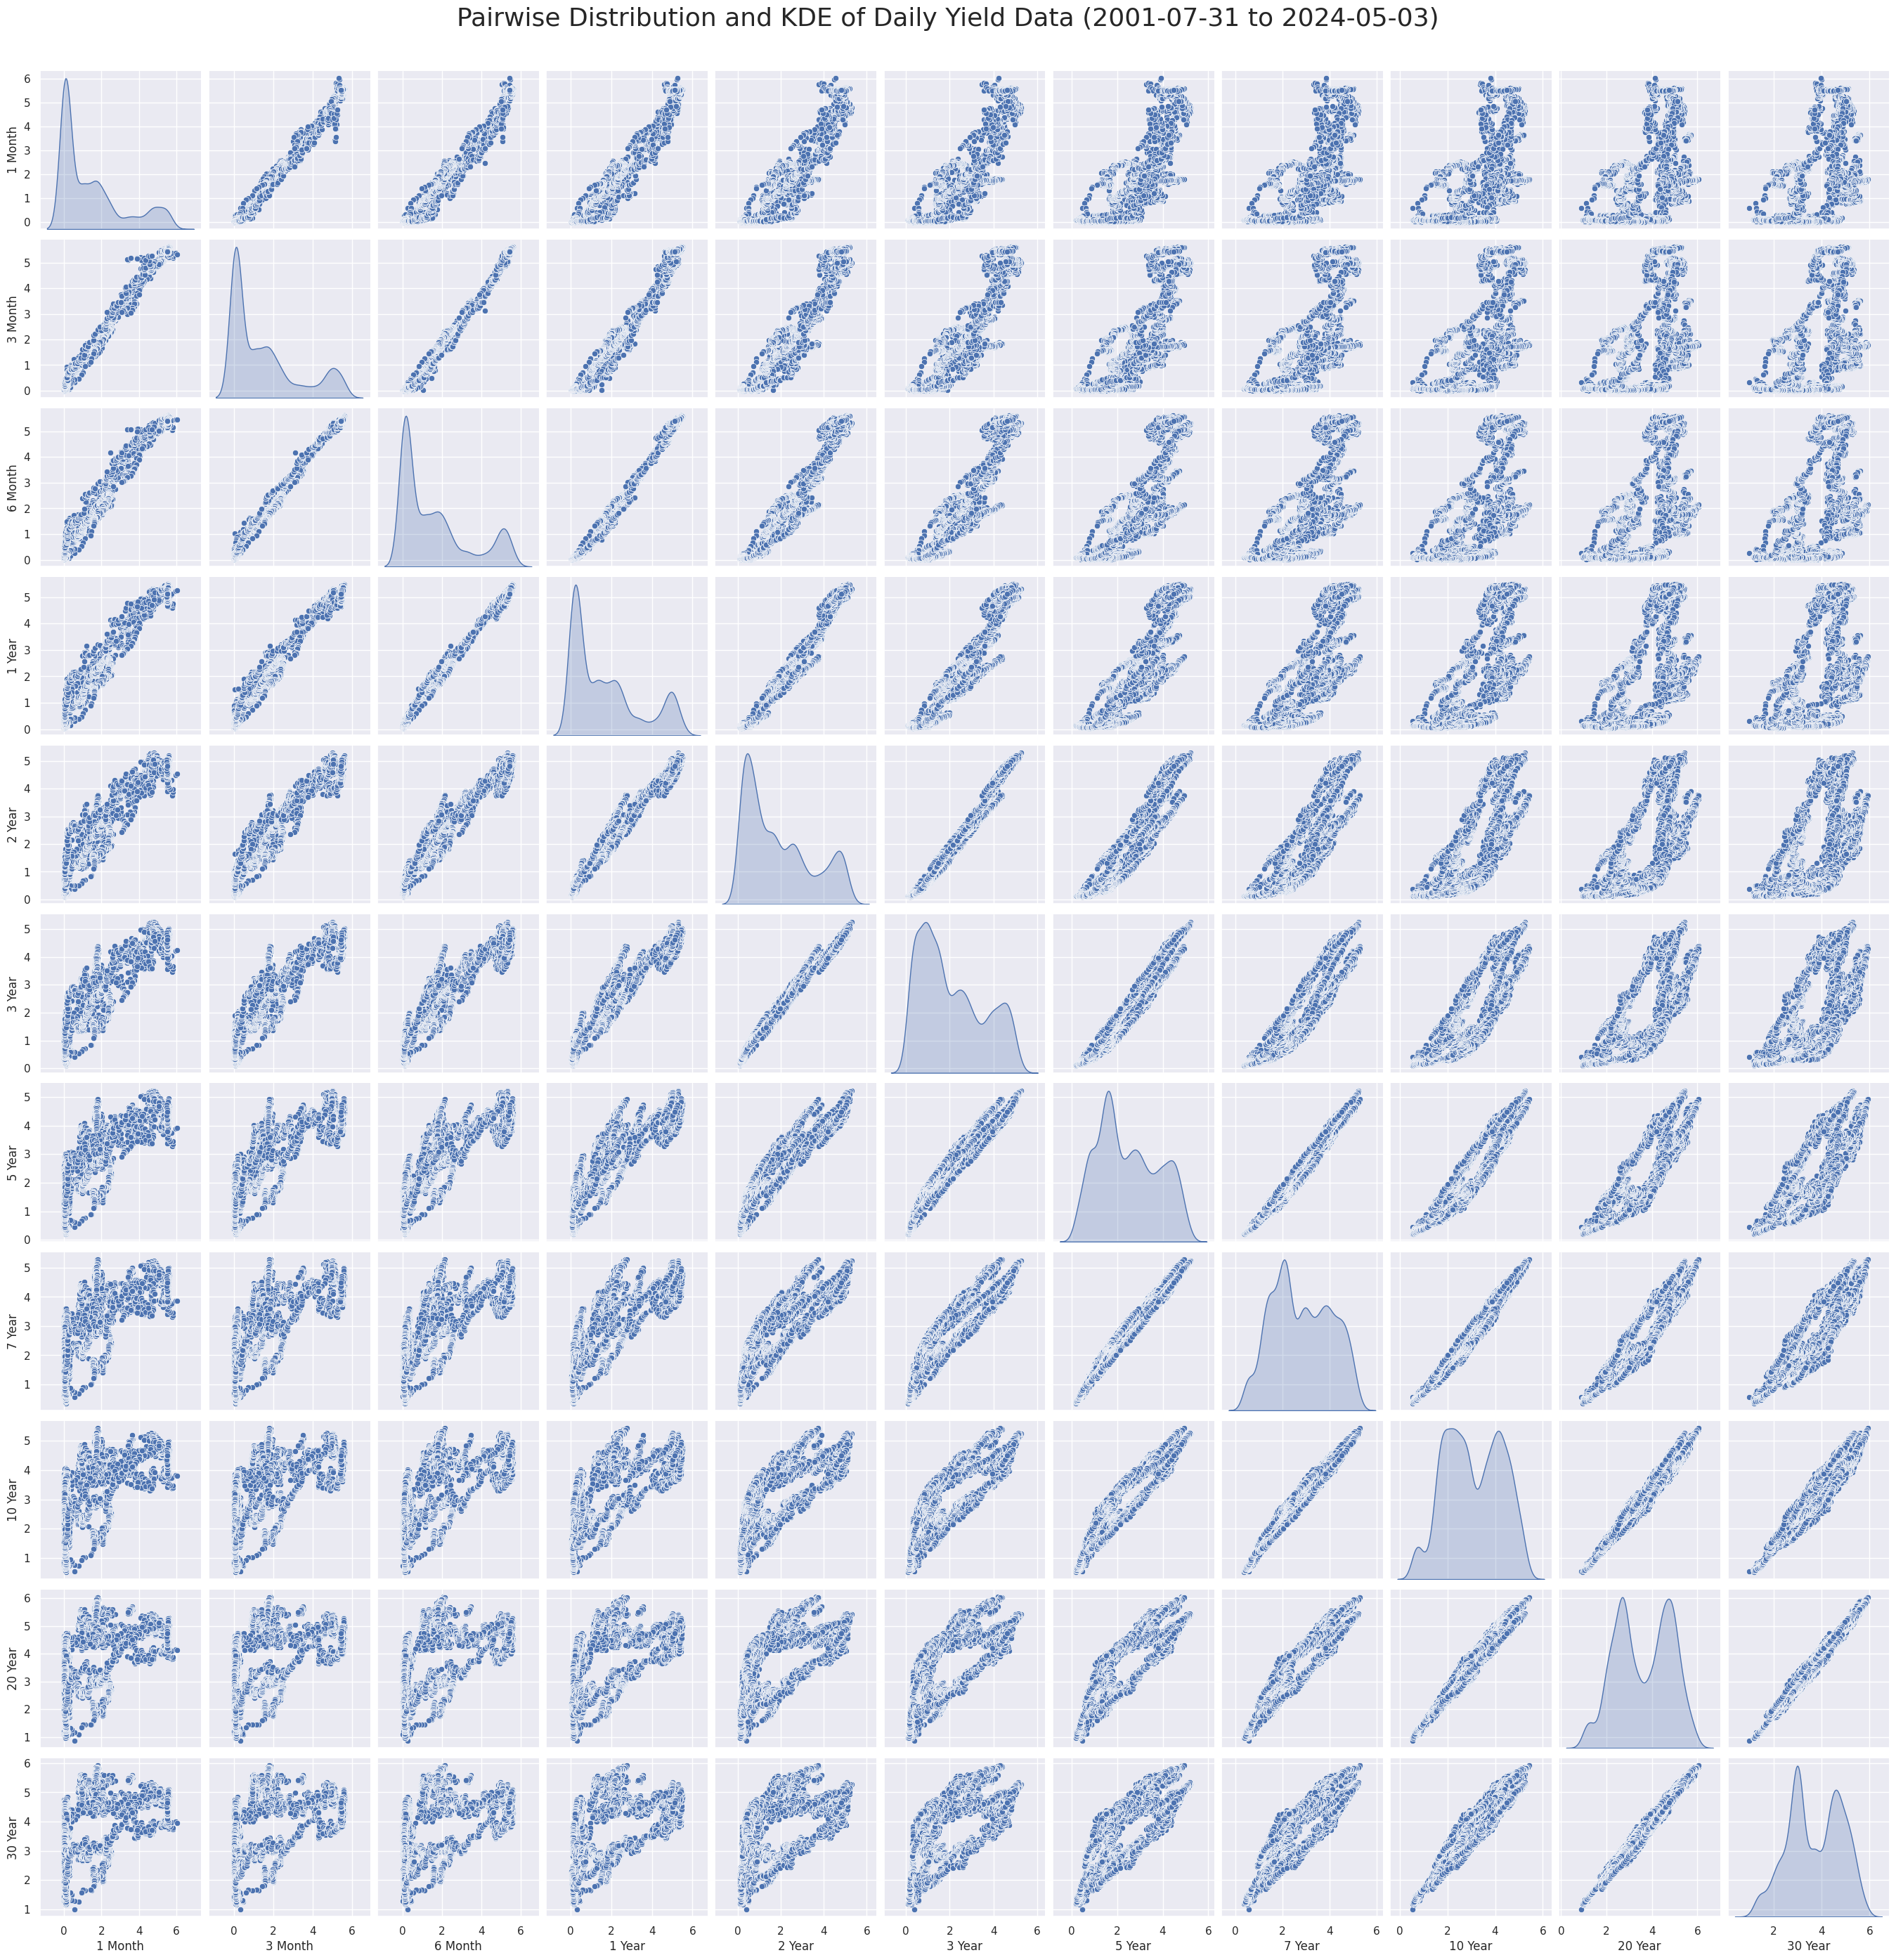
\includegraphics[width=1\textwidth]{gfx/m1l2_notes_fig2_pairplot.png}
    \caption{Phân phối theo cặp và Ước lượng mật độ hạt nhân (KDE) của dữ liệu lợi suất hàng ngày}
    \label{fig:m1l2_notes_fig2_pairplot}
\end{figure}

Biểu đồ cặp (pairplot) ở trên hiển thị mối quan hệ giữa Trái phiếu Kho bạc Hoa Kỳ ở các kỳ hạn khác nhau. Trên đường chéo, chúng ta có thể thấy ước lượng mật độ hạt nhân (kernel density estimation - KDE) của từng mức lợi suất trong khi các biểu đồ nằm ngoài đường chéo hiển thị các biểu đồ phân tán (scatterplots) cho mỗi cặp.

Điều đầu tiên chúng ta nhận thấy là KDE của các mức lợi suất có dạng đa đỉnh (multimodal). Điều này phản ánh tác động của các chế độ kinh tế, chu kỳ, thay đổi chính sách và các sự kiện quan trọng khác nhau lên lợi suất.

Thêm vào đó, các biểu đồ phân tán cho thấy mối tương quan dương mạnh mẽ giữa các mức lợi suất. Cụ thể hơn, các lợi suất có kỳ hạn gần nhau có mối tương quan hoàn hảo (gần bằng 1) trong khi các lợi suất xa nhau vẫn có tương quan dương mặc dù không hoàn hảo.

Hãy trực quan hóa các lợi suất tại một ngày cụ thể:

\begin{lstlisting}[language=Python]
In [8]: # Figure 3
        def plot_yield_curve(date):
            maturities = ['1M', '3M', '6M', '1Y', '2Y', '3Y', '5Y', '7Y', '10Y', '20
            fig, ax = plt.subplots(figsize=(12, 6))
            ax.plot(maturities, yields.loc[date], marker='D', label='Yield Curve at 
            
            ax.set_yticklabels(['{:.2f}%'.format(y) for y in ax.get_yticks()])
            ax.set_xticks(range(len(maturities)))
            ax.set_xticklabels(maturities)
            
            # Add labels and title
            ax.set_xlabel('Maturity')
            ax.set_ylabel('Yield')
            ax.set_title('Treasury Yield Curve')
            
            fig.legend(loc = [0.69, 0.14])
            
            # Show the plot
            plt.grid(True)
            plt.show()

        plot_yield_curve('2020-01-03')
\end{lstlisting}

\begin{lstlisting}[language=Python]
/tmp/ipykernel_17/2521112310.py:8: UserWarning: set_ticklabels() should only 
be used with a fixed number of ticks, i.e. after set_ticks() or using a Fixe
dLocator.
  ax.set_yticklabels(['{:.2f}%'.format(y) for y in ax.get_yticks()])
\end{lstlisting}

\begin{figure}[htbp]
    \centering
    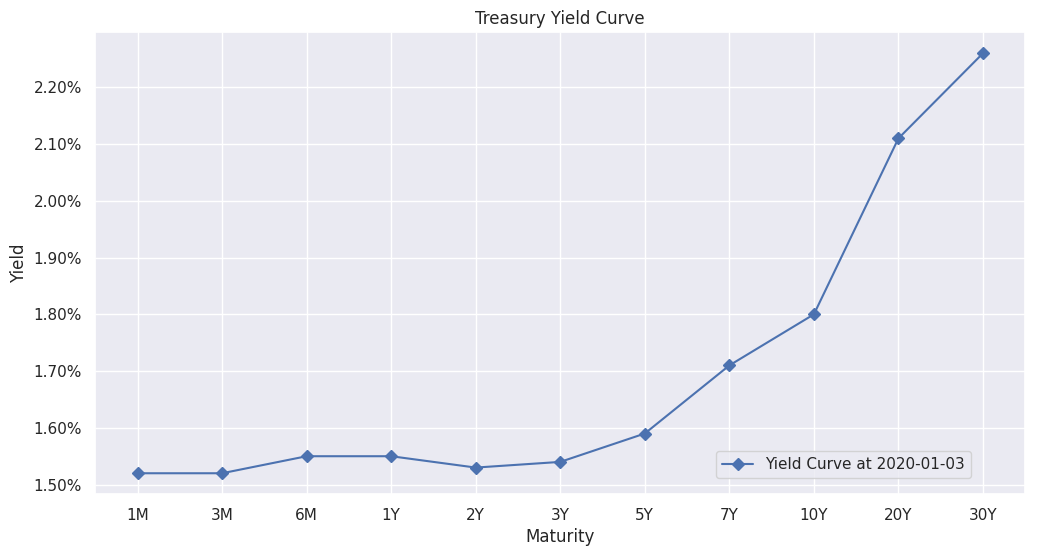
\includegraphics[width=1\textwidth]{gfx/m1l2_notes_fig3_yield_curve_2020.png}
    \caption{Đường cong lợi suất Trái phiếu Kho bạc ngày 03-01-2020}
    \label{fig:m1l2_notes_fig3_yield_curve_2020}
\end{figure}

Bài tập 2
Biểu đồ trên hiển thị tất cả các lợi suất tại ngày 2020-01-03. Hãy tìm (một hoặc hai) ngày cụ thể giúp bạn vẽ lại biểu đồ trên hai lần: một lần cho một đường cong dẹt (flattened curve) và một lần cho một đường cong đảo ngược (inverted curve). Lập luận xem các đường cong dẹt và đường cong đảo ngược tương ứng với các giai đoạn cụ thể nào của Hình 1 (trong một số trường hợp, các đường lợi suất kết hợp trông rất mỏng). Tại sao những ngày đó lại quan trọng?

\subsection[Hình dạng của Đường cong Lợi suất]{Hình dạng của Đường cong Lợi suất (The Shape of the Yield Curve)}

Bằng cách kiểm tra Hình 3 cùng với các hình ảnh mà bạn đã tạo ra khi trả lời Bài tập 2, bạn đã quan sát thấy rằng các yếu tố (rõ ràng nhất) định hình đường cong lợi suất là (Rebonato):
1. Mức độ (level) tổng thể của đường cong lợi suất, biểu thị mức lãi suất đang cao hay thấp như thế nào.
2. Độ dốc (slope) của đường cong lợi suất, cho biết đường cong dốc, phẳng hay đảo ngược như thế nào.

Thông thường, chúng ta có thể giải thích khoảng 90\% sự biến thiên của đường cong thông qua mức độ và độ dốc (Oprea). Để phân tích kỹ lưỡng hơn, người ta cần tính đến yếu tố thứ 3: Độ cong (curvature), đây là thước đo cách thức phần giữa của đường cong (lãi suất trung hạn) hoạt động so với lãi suất ngắn hạn và dài hạn.

Vì mục đích của bài học này, chúng ta sẽ nhấn mạnh vào hai yếu tố đầu tiên.

\subsubsection[Mức độ của Đường cong]{Mức độ của Đường cong (Level of the Curve)}

Mức độ gắn liền với những dịch chuyển song song trong toàn bộ đường cong lợi suất. Về cơ bản, nó ảnh hưởng đến tất cả giá trái phiếu bất kể kỳ hạn với biên độ (gần như) giống nhau. Những dịch chuyển này được thúc đẩy bởi các yếu tố kinh tế vĩ mô như lạm phát, các sự kiện địa chính trị, thay đổi trong chính sách tiền tệ, v.v.

Chúng ta sẽ xem xét Cuộc khủng hoảng Thị trường Trái phiếu năm 1994, còn được gọi là Cuộc Thảm sát Trái phiếu Vĩ đại (Great Bond Massacre). Tác nhân chính dẫn đến sự sụp đổ của trái phiếu là quyết định của Fed khởi xướng một đợt tăng lãi suất. Vào tháng 2 năm 1994, Fed đã nâng lãi suất quỹ từ 3.00\% lên 3.25\%. Trong suốt cả năm, Fed tiếp tục tăng lãi suất theo từng bước, đạt 5.5\% vào tháng 2 năm 1995. Động lực chính đằng sau quyết định của Fed là kỳ vọng lạm phát do sự mở rộng kinh tế nhanh chóng vào năm 1993.

Hơn nữa, trước năm 1994, mức chênh lệch (spread) giữa lãi suất ngắn hạn và dài hạn là hơn 4 điểm phần trăm, dẫn đến việc nhiều nhà đầu tư ở các vị thế đòn bẩy vay ngắn hạn và đầu tư vào các trái phiếu dài hạn hơn. Đương nhiên, những đợt tăng lãi suất đột ngột đã khiến những nhà đầu tư này (trong số những người khác) mất cảnh giác, buộc họ phải tháo gỡ vị thế của mình, dẫn đến một đợt bán tháo trên thị trường trái phiếu.

\begin{lstlisting}[language=Python]
In [9]: # Figure 4
        from matplotlib.gridspec import GridSpec
        
        # Preparing the data
        bond_market_crash = yields.loc['1994-01-03':'1994-11-30'].iloc[::] * 100
        resampled_monthly_bond_market_crash = bond_market_crash.resample('M').last()
        resampled_monthly_bond_market_crash_ticks = resampled_monthly_bond_market_cr
        
        # Creating the plt object
        fig = plt.figure(figsize=(16, 12))
        gs = GridSpec(2, 2, height_ratios=[1, 1.5])
        
        # First row, first column
        ax1 = fig.add_subplot(gs[0, 0])
        ax1.plot(bond_market_crash, alpha=0.7)
        ax1.set_title('Treasury Yields across time - Graph 1')
        ax1.set_xlabel('Date')
        ax1.set_ylabel('Yield (%)')
        ax1.tick_params(axis='x', rotation=45)
        
        # First row, second column
        ax2 = fig.add_subplot(gs[0, 1])
        ax2.bar(resampled_monthly_bond_market_crash_ticks, resampled_monthly_bond_ma
        ax2.set_title('Mean Yields across time - Graph 2')
        ax2.set_xlabel('Date')
        ax2.set_ylabel('Average Yield (%)')
        ax2.tick_params(axis='x', rotation=45)
        
        # Second row
        ax3 = fig.add_subplot(gs[1, :])
        for i in range(len(resampled_monthly_bond_market_crash)):
            date = resampled_monthly_bond_market_crash_ticks[i]
            resampled_monthly_bond_market_crash.iloc[i].plot(ax=ax3, alpha=0.7, l
        
        ax3.set_title('Yield Curves at the end of each month - Graph 3')
        ax3.set_xlabel('Maturity')
        ax3.set_ylabel('Yield (%)')
        ax3.legend(title='Date', loc='center left', bbox_to_anchor=(1, 0.5))
        ax3.tick_params(axis='x', rotation=45)
        
        plt.tight_layout()
        plt.show()
\end{lstlisting}

\begin{lstlisting}[language=Python]
/tmp/ipykernel_17/3704098406.py:7: FutureWarning: 'M' is deprecated and will
be removed in a future version, please use 'ME' instead.
  resampled_monthly_bond_market_crash = bond_market_crash.resample('M').last
()
\end{lstlisting}

\begin{figure}[htbp]
    \centering
    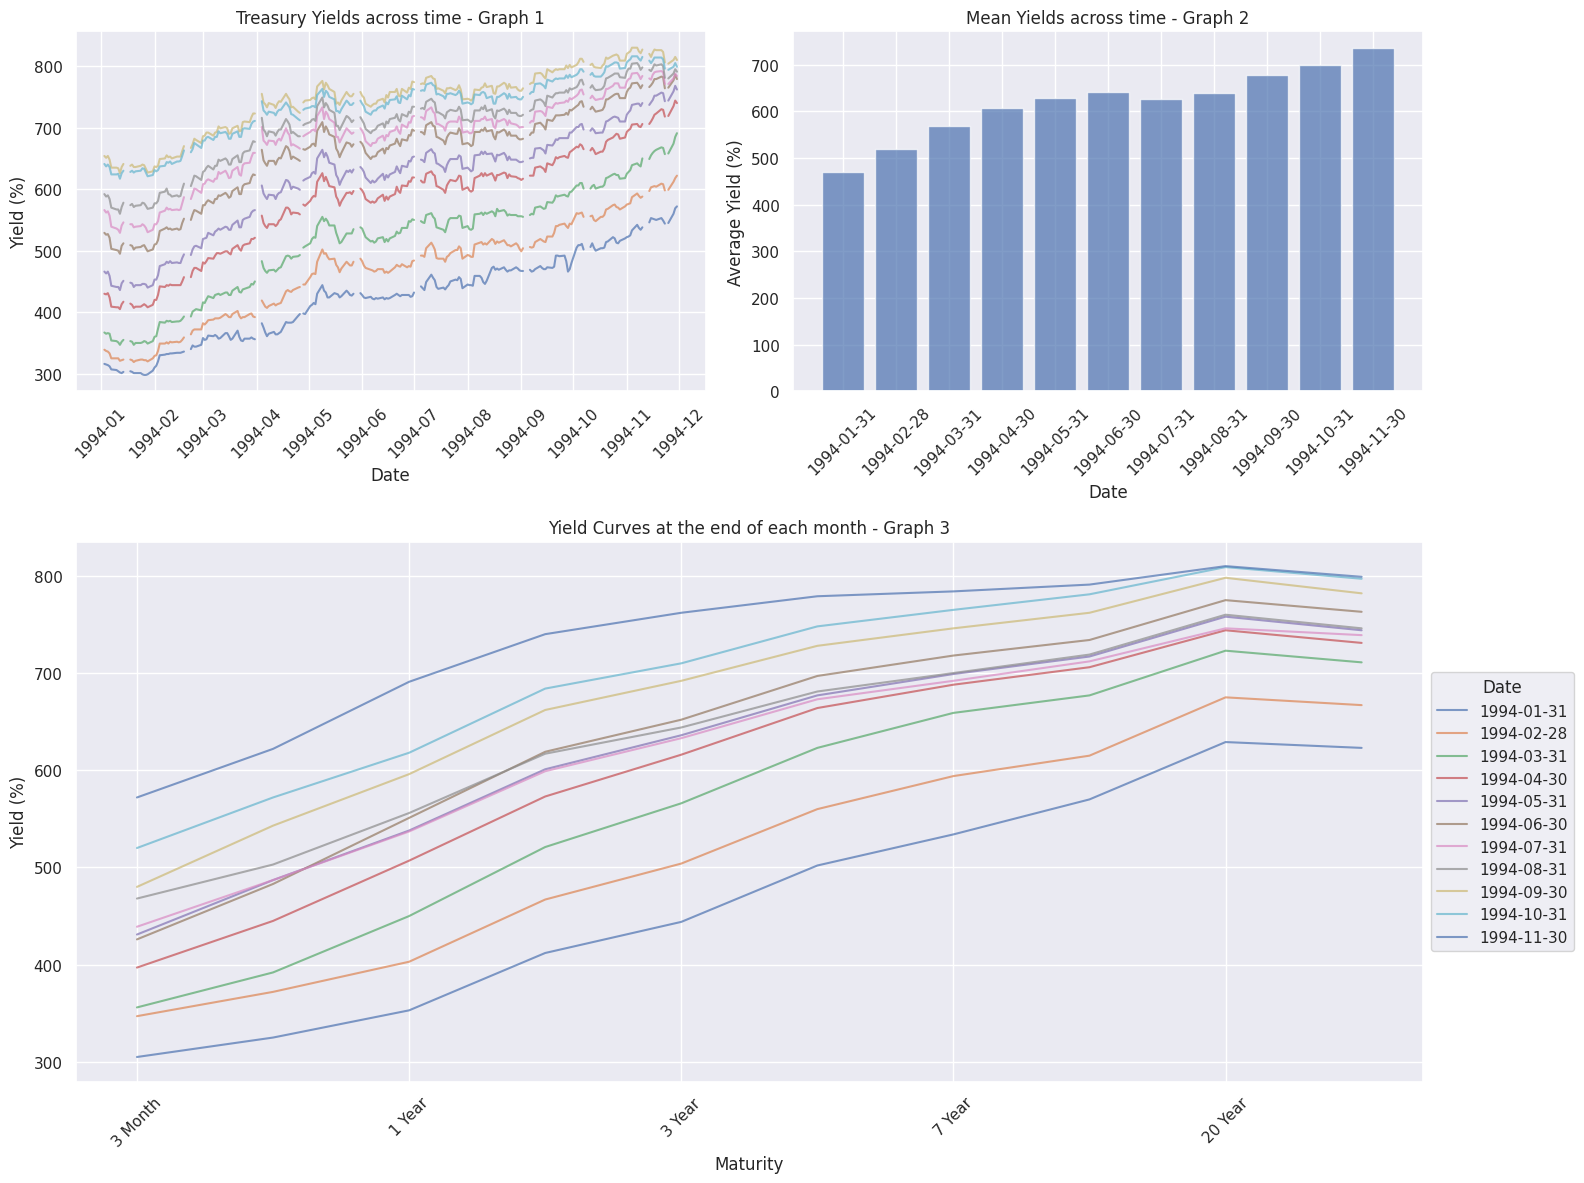
\includegraphics[width=1\textwidth]{gfx/m1l2_notes_fig4_bond_crash_1994.png}
    \caption{Khủng hoảng Thị trường Trái phiếu 1994}
    \label{fig:m1l2_notes_fig4_bond_crash_1994}
\end{figure}

Trong Hình 4, người ta có thể thấy sự dịch chuyển tăng lên nhất quán của lợi suất qua tất cả các kỳ hạn. Cụ thể trong Đồ thị 3, chúng ta quan sát thấy mọi đường cong lợi suất vào cuối mỗi tháng trong năm 1994 (ngày cuối cùng của mỗi tháng được chọn ngẫu nhiên để đại diện cho tháng đó). Đây là một ví dụ điển hình về sự thay đổi mức độ của các lợi suất, nơi toàn bộ đường cong đang di chuyển lên trên mỗi tháng trong khi vẫn giữ nguyên độ dốc của nó.

\subsubsection[Độ dốc của Đường cong Lợi suất]{Độ dốc của Đường cong Lợi suất (Slope of the Yield Curve)}

Độ dốc của đường cong lợi suất thường chỉ sự chênh lệch lợi suất giữa trái phiếu dài hạn và ngắn hạn. Chúng ta thường sử dụng sự chênh lệch giữa trái phiếu 10 năm và 2 năm hoặc giữa trái phiếu 30 năm và 3 tháng, nhưng tùy thuộc vào bối cảnh, người ta có thể chọn các kỳ hạn khác nhau. Độ dốc có thể được phân loại thành:
\begin{enumerate}
    \item Độ dốc dương (positive slope), còn được gọi là đường cong lợi suất bình thường (normal yield curve), xảy ra khi lợi suất dài hạn cao hơn lợi suất ngắn hạn. Đây là kịch bản "bình thường" vì chúng ta kỳ vọng rằng rủi ro bổ sung khi nắm giữ trái phiếu dài hạn sẽ được bù đắp bằng lợi nhuận cao hơn so với trái phiếu ngắn hạn.
    \item Độ dốc phẳng (flat slope): lợi suất ngắn hạn và dài hạn là tương đương nhau.
    \item Độ dốc âm (negative slope), còn được gọi là đường cong lợi suất đảo ngược (inverted yield curve). Nó xảy ra khi lợi suất ngắn hạn cao hơn lợi suất dài hạn.
\end{enumerate}

Như chúng ta đã thấy cho đến hiện tại, độ dốc có thể dễ dàng nhìn thấy trong biểu đồ đường cong lợi suất. Nhưng còn động lực học của những thay đổi độ dốc thì sao?

Giả sử chúng ta đang ở vị trí mà đường cong lợi suất là bình thường. Từ điểm này, độ dốc có thể trở nên dốc hơn (steepen) hoặc phẳng ra (flatten), và trong mỗi trường hợp, điều này có thể xảy ra theo nhiều cách:

\begin{enumerate}
    \item Trở nên dốc hơn (Steepening)
    \begin{itemize}
        \item Đường cong dốc lên do thị trường giá lên (Bull steepening): lãi suất ngắn hạn giảm nhanh hơn lãi suất dài hạn
        \item Đường cong dốc lên do thị trường giá xuống (Bear steepening): lãi suất dài hạn tăng nhanh hơn lãi suất ngắn hạn
    \end{itemize}
    \item Phẳng ra (Flattening)
    \begin{itemize}
        \item Đường cong dẹt đi do thị trường giá lên (Bull flattening): lãi suất dài hạn giảm nhanh hơn lãi suất ngắn hạn
        \item Đường cong dẹt đi do thị trường giá xuống (Bear flattening): lãi suất ngắn hạn tăng nhanh hơn lãi suất dài hạn
    \end{itemize}
\end{enumerate}

Trong Hình 5, bạn có thể thấy một sự thể hiện trực quan về động lực học phẳng ra của đường cong.

\begin{lstlisting}[language=Python]
In [10]: # Figure 5
         # Preparing the data
         bear_flattening = yields['2004-06-01':'2006-06-30'].resample('3M').last()
         bear_flattening.index = bear_flattening.index.strftime('%Y-%m-%d')
         
         bull_flattening = yields['2010-01-01':'2012-06-30'].resample('4M').last()
         bull_flattening.index = bull_flattening.index.strftime('%Y-%m-%d')
         
         # Creating the plt object
         fig, (ax1, ax2) = plt.subplots(1, 2, figsize=(16, 6))
         
         # Bear flattening graph
         for i in range(len(bear_flattening)):
             date = bear_flattening.index[i]
             ax1.plot(bear_flattening.columns, bear_flattening.iloc[i, :], alpha=0.7, 
         
         ax1.set_title('Bear Flattening: 2004 - 2006')
         ax1.set_xlabel('Maturity')
         ax1.set_ylabel('Yield (%)')
         ax1.legend(title='Date', loc='center left', bbox_to_anchor=(1, 0.5))
         ax1.tick_params(axis='x', rotation=45)
         
         # Bull flattening graph
         for i in range(len(bull_flattening)):
             date = bull_flattening.index[i]
             ax2.plot(bull_flattening.columns, bull_flattening.iloc[i, :], alpha=0.7,
         
         ax2.set_title('Bull Flattening: 2010 - 2012')
         ax2.set_xlabel('Maturity')
         ax2.set_ylabel('Yield (%)')
         ax2.legend(title='Date', loc='center left', bbox_to_anchor=(1, 0.5))
         ax2.tick_params(axis='x', rotation=45)
         
         plt.tight_layout()
         plt.show()
\end{lstlisting}

\begin{figure}[htbp]
    \centering
    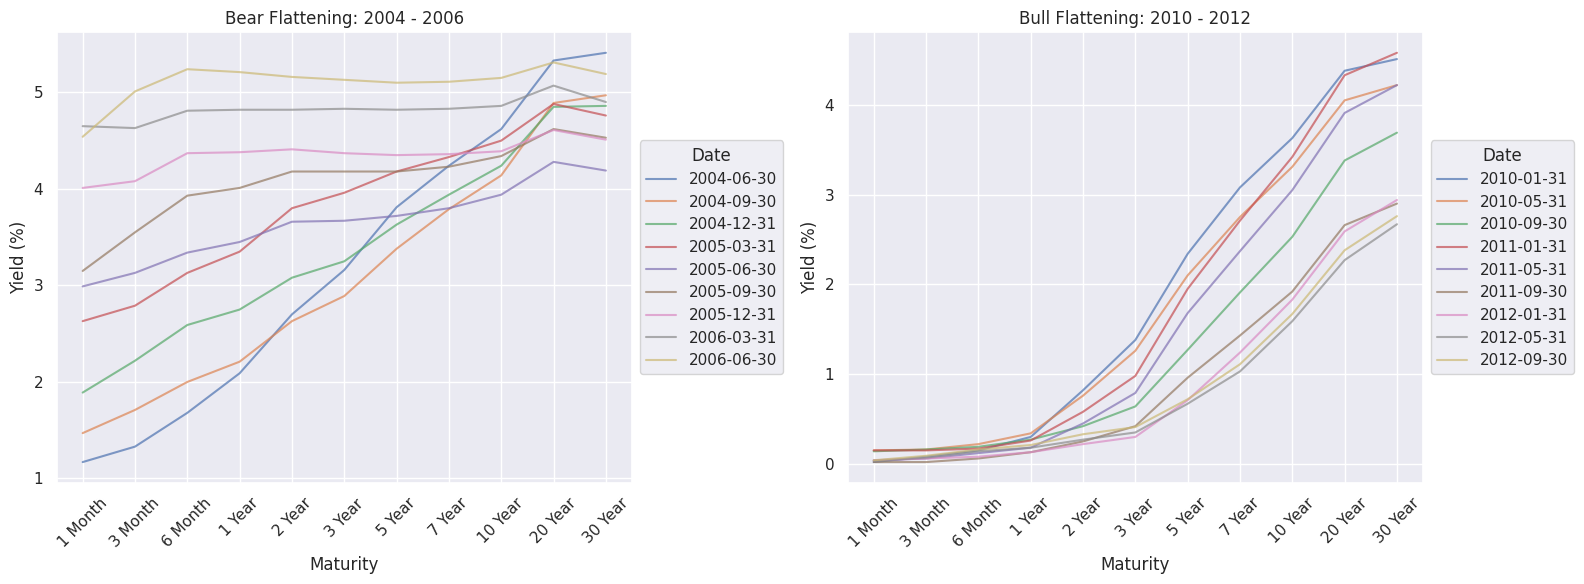
\includegraphics[width=1\textwidth]{gfx/m1l2_notes_fig5_flattening.png}
    \caption{Động lực học phẳng ra của đường cong (Bear Flattening và Bull Flattening)}
    \label{fig:m1l2_notes_fig5_flattening}
\end{figure}

Bài tập 3
Vẽ lại Hình 5 để minh họa các hiện tượng đường cong dốc lên do thị trường giá lên (bull steepening) và giá xuống (bear steepening). Tìm kiếm các khoảng thời gian tương ứng với sự dốc lên của đường cong lợi suất bằng cách tra cứu trực tuyến hoặc trong các sách giáo khoa học thuật, và sử dụng đoạn mã được cung cấp để chứng minh các động lực học của sự dốc lên này. Lập luận về các điều kiện kinh tế và phản ứng của Fed trong những khoảng thời gian này. Dán biểu đồ vào diễn đàn cùng với một đoạn văn nhỏ giải thích những gì chúng ta nhìn thấy.

Bài tập 4
Chứng minh tầm quan trọng của chênh lệch giữa trái phiếu 10 năm và 2 năm. Tạo một biểu đồ có trục y kép (double y-axis plot) trong đó bạn xếp chồng (superimpose) chỉ số S\&P500 lên mức chênh lệch giữa hai trái phiếu này.

\section[Kết luận]{Kết luận (Conclusion)}

Thông qua việc phân tích và trực quan hóa thực hành bằng Python và FRED API, chúng ta đã xem xét động lực học của đường cong lợi suất qua thời gian. Chúng ta đã khám phá cách các yếu tố như mức độ và độ dốc định hình đường cong lợi suất và cách những thành tố này phản ánh cũng như ảnh hưởng đến các điều kiện kinh tế rộng lớn hơn.

Những điểm chính rút ra bao gồm:
\begin{itemize}
    \item Tầm quan trọng của dữ liệu chính phủ mở đối với hoạt động nghiên cứu, hoạch định chính sách và sự hiểu biết của công chúng về các xu hướng kinh tế
    \item Tầm quan trọng của đường cong lợi suất với tư cách là một chỉ báo kinh tế, bao gồm nhiều hình dạng khác nhau của nó (bình thường, phẳng và đảo ngược) và những hình dạng đó có thể biểu thị điều gì về các kỳ vọng kinh tế
    \item Khái niệm đường cong lợi suất dốc lên và dẹt đi cũng như cách những biến động này có thể được phân loại là "bull" (giá lên) hoặc "bear" (giá xuống) tùy thuộc vào những thay đổi lãi suất cơ bản
\end{itemize}

\section*{Tài liệu tham khảo (References)}
\begin{itemize}
    \item Rebonato, Riccardo. Bond Pricing and Yield Curve Modeling: A Structural Approach. Cambridge University Press, 2018.
    \item Oprea, Andreea, The Use of Principal Component Analysis (PCA) in Building Yield Curve Scenarios and Identifying Relative-Value Trading Opportunities on the Romanian Government Bond Market, Journal of Risk and Financial Management, 2022, 15(6), 247
\end{itemize}

Copyright 2024 WorldQuant University. This content is licensed solely for personal use. Redistribution or publication of this material is strictly prohibited.
